\newpage

\section{Coulomb-Nuclear Interference}
\label{sec:coulomb}

\> outline for this section

\> reason for using 90m data
\> different ways of using 1000 and 90m data: combined (democratically), differential (tensions), combined (each DS used where strong)

%----------------------------------------------------------------------------------------------------

\subsection{Theoretical Framework}
\label{sec:cni framework}

In this section the different components of the combined elastic scattering amplitude, already briefly outlined in the introduction, are discussed in more detail. In particular, the possible choices for theoretically unknown terms are explained.

%------------------------------------------------------------------
\subsubsection{Coulomb Amplitude}
\label{sec:cni coulomb}
%
The Coulomb amplitude can be calculated from QED (e.g.~Section 3.2 in \cite{block06}), using empirical electric and magnetic form factors of the proton (e.g.~\cite{puckett10}). It can be shown (e.g.~Section 1.3.1 in~\cite{jan_thesis}) that, at low $|t|$, the effect of both form factors can be described by a single function ${\cal F}$. 

\TODO{Add formula}

\TODO{Choice of FF no impact on final results}

%------------------------------------------------------------------
\subsubsection{Nuclear Amplitude}
\label{sec:cni nuclear}
%
Since the nuclear amplitude can presently not be calculated from first principles, its phenomenological description will be discussed.

\vskip3mm
\hbox to\hsize{\bf Modulus\hfil}

The modulus is closely related to the differential cross-section and thus strongly constrained by experimental observations outside the Coulomb and CNI region. Following especially~\cite{8tev-90m}, the modulus for $|t|~\lesssim~0.2$, i.e. well below the diffractive minimum, will be parametrised as:
\begin{equation}
\label{eq:nuc mod}
| {\cal A}^{\rm N}(t) | = a \exp\left( \sum\limits_{n}^{N_b} b_n t^n \right)\ ,
\end{equation}
%\TODO{for $|t| < 0.2$, what about higher $|t|$'s?}\\
where $N_b$ gives the number of free parameters in the exponent. This implicitly extends the exponential behaviour to the regions where the (pure nuclear) cross-section cannot be observed. Although there is no rigorous justification, and therefore it stands as an assumption, it is compatible with many theoretical models.

\TODO{considering $N_b = $ 1, 2 and 3 parameters, with more parameters no improvement of $\chi^2$}

\TODO{anchored to $90\un{m}$ data at $|t| > 0.2\un{GeV^2}$ for stability of integrations in Eq.~(\ref{eq:int kl}); high t part has no effect on final results}

\TODO{This parametrisation assumes that Coulomb effects are small, which is not unreasonable, the expected order is few percent}

\vskip3mm
\hbox to\hsize{\bf Phase\hfil}

For the phase of the nuclear amplitude, there is little experimental guidance and therefore several theory-motivated choices will be assumed and tested.

\begin{itemize}
% ***
\item A {\it constant phase} is obviously the simplest choice:
%
\begin{equation}
\label{eq:nuc phase con}
\arg {\cal A}^{\rm N}(t) = p_0 = \hbox{const.}
\end{equation}
Note that this is equivalent to a strict proportionality of real and imaginary part of the amplitude at all $t$.
%
% ***
\item The {\it standard phase} parametrisation,
\begin{equation}
\label{eqn:nuc phase std}
\arg {\cal A}^{\rm N}(t) = p_{0} + \arctan \left(\frac{|t|-|t_{0}|}{\tau}\right) -  \arctan \left(\frac{-|t_{0}|}{\tau}\right) \: ,
\end{equation}
implements the main features of many theoretical models -- almost imaginary amplitude in the forward direction ($p_0 \approx \pi/2$) while almost purely real in the (first) diffraction dip 
($\arg {\cal A}^{\rm N}(t) \approx \pi$ at $t = t_{0}$). \TODO{[to be corrected]}

% ***
%
\item The parametrisation by {\em Bailly et al.}~\cite{bailly87} \TODO{motivation for this option}
\begin{equation}
\label{eq:nuc phase bai}
	%\arg {\cal A}^{\rm N}(t) = {\pi\over 2} - \arctan {\rho_0\over 1 - {t\over t_{\rm d}}},\ \rho_0 = {1\over \tan p_0}
	\arg {\cal A}^{\rm N}(t) = \arctan \left[ \tan p_0 \left(1 - {t\over t_{\rm d}} \right) \right]\ ,
\end{equation}
where $p_0$ determines the phase value at $t=0$ and $t_{\rm d} \approx -0.53\un{GeV^2}$ gives the position of the diffractive minimum at $8\un{TeV}$ (preliminary result from $90\un{m}$ data).
%
% ***
\item The {\it peripheral phase} \cite{kl94} \TODO{newer ref - if we ever get one} provides an alternative to the above descriptions. Its parametrisation

\TODO{update values, range?}\\
\TODO{if range used: several options with different level of peripherality as assumption - the RMS of b el was initially fixed by Vojtech - it is a cause not consequence}

\begin{equation}
\label{eq:nuc phase per}
\arg {\cal A}^{\rm N}(t) = p_0 - A \exp\left[ \kappa \left( \log {t\over t_{\rm m}} - {t\over t_{\rm m}} + 1 \right) \right]
\end{equation}
results in a peak at $t_{\rm m} \approx -0.310\un{GeV^2}$, with amplitude $A \approx 5.53$ and width controlled by $\kappa \approx 4.01$.
\end{itemize}

\begin{figure*}
\begin{center}
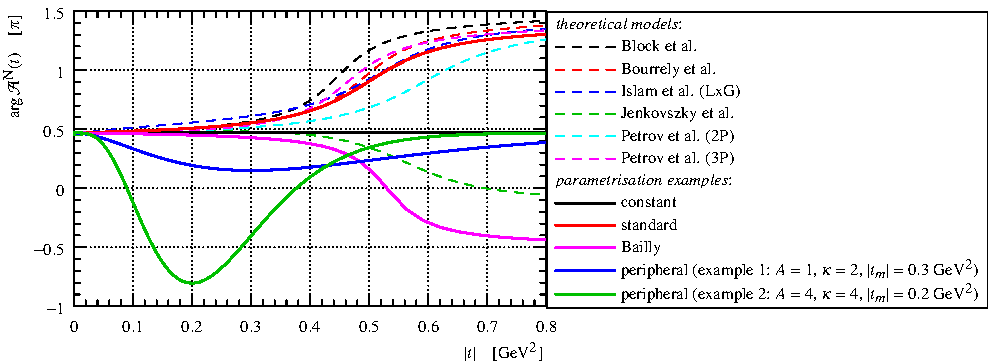
\includegraphics{fig/hadronic_phase_illustration.pdf}
\caption{Illustration of hadronic-phase forms. The dashed lines correspond to predictions by theoretical models as provided by \cite{elegent}. The solid lines give typical examples of parametrisations used in the study, all at the same value of $\rho = 0.12$.}
\label{fig:phase illustration}
\end{center}
\end{figure*}

It should be noted that the phase has decisive influence on the amplitude behaviour in the space of impact parameter, $b$, see e.g.~Section 3 in~\cite{klk02}. It can be quantified by evaluating the root-mean-squares (RMS) of $b$ for elastic and inelastic collisions. The constant and standard phase lead to elastic collisions more central (smaller RMS) than the inelastic ones. The peripheral phase can yield a description with the opposite hierarchy, which is argued more natural by some authors (e.g. Section~4 in~\cite{kl96}).

%------------------------------------------------------------------
\subsubsection{Coulomb-Nuclear Interference Formulae}
\label{sec:cni interference}

The {\bf simplified West-Yennie formula (SWY)} \cite{wy68} is derived in the framework of perturbative QFT by evaluating the lowest-order Feynman diagrams that comprise both nuclear and Coulomb interactions. In this approach, the interference is reduced to an additional phase between the Coulomb and nuclear amplitudes. Moreover, several approximations were used in the derivation. First, in order to avoid integrating over off-mass-shell contributions to the nuclear amplitude (purely known), very slow variation of the nuclear amplitude phase was assumed: $\arg {\cal A}^{\rm N} \approx \hbox{const}$. Then, in order to obtain a closed-form expression, the exponential slope of the nuclear modulus
\begin{equation}
B^{\rm N}(t) = {\d \log |{\cal A}^{\rm N}|^2 \over \d t}
\end{equation}
was assumed constant. The original formula did not contain the electromagnetic form factor ${\cal F}$, it was added later by hand:
\begin{equation}
\label{eq:int swy}
	\begin{aligned}
		{\d\sigma\over \d t}^{\rm C+N} &= {\pi (\hbar c)^2 \over s p^2} \left | {\alpha s\over t} {\cal F}^2 \e^{\I\alpha \Phi(t)} + {\cal A}^{\rm N} \right |^2\ ,\cr
		\Phi(t) &= - \left( \log {B^{\rm N} |t|\over 2} + \gamma \right)\ ,\cr
	\end{aligned}
\end{equation}
where $\gamma \doteq 0.577$ is the Euler constant. Despite the many limitations, the formula has extensively been used in past data analyses. For backward-comparison reasons we consider it also in this report.

The {\bf Kundr\' at-Lokaj\' i\v cek formula (KL)} \cite{kl94} was derived in an impact parameter formalism and it is based on the additivity of eikonals. The derivation poses no limitations on nuclear amplitude and the formula naturally incorporates the electromagnetic form-factor. In this treatment, the interference effect goes beyond a single phase, the $\Psi$ quantity is complex, in general:
\begin{equation}
\label{eq:int kl}
	\begin{aligned}
		{\d\sigma\over \d t}^{\rm C+N} &= {\pi (\hbar c)^2 \over s p^2} \left | {\alpha s\over t} {\cal F}^2 + {\cal A}^{\rm N} \e^{\I\alpha \Psi(t)} \right |^2\ ,\cr
		\Psi(t) &= 
			- \int \d t'\, \log {t'\over t} {\d\phantom{t'}\over \d t'} {\cal F}^2(t') \cr
		&\phantom{=} + \int \d t' \left( {{\cal A}^{\rm N}(t') \over {\cal A}^{\rm N}(t)} - 1 \right) { I(t, t')\over 2\pi }
			\ ,\cr
		I(t, t') &= \int_0^{2\pi} \d\phi\ {{\cal F}^2(t'')\over t''}\ , \cr
		t'' &= t + t' + 2\sqrt{t\, t'} \cos\phi\ ,\cr
	\end{aligned}
\end{equation}
where the $t$ integrations go over the entire kinematically allowed region.

Calculation engine \cite{elegent}, using form-factor of Puckett et al.~\cite{puckett10}

\TODO{Show an ``exploration'' plot to explain the C+CNI reaction to changing $p_0$ (low $|t|$) and higher orders (higher $|t|$) -- could be very instructive}

\begin{figure*}
\begin{center}
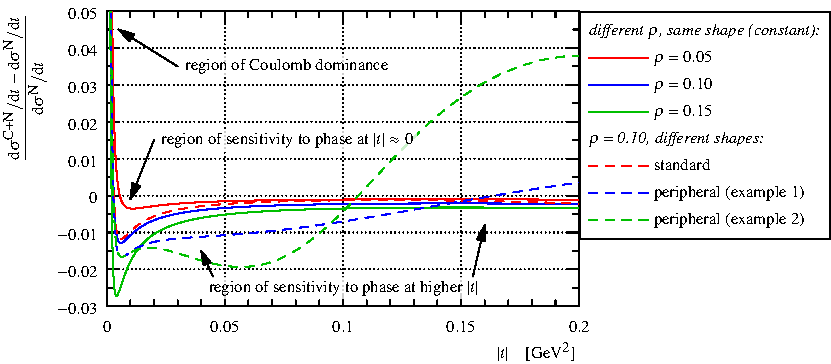
\includegraphics{fig/cni_effect_illustration.pdf}
\caption{\TODO{caption} Illustration of effects due to the Coulomb interaction, using KL formula (SWY formula misses the effects at higher $|t|$). Different $|t|$ regions probe different parts of the nuclear phase. Difference between constant and standard (and also Bailly) very small -- all have small derivatives of the phase at low $|t|$. The higher $|t|$ effects for peripheral phase are of the order of several percents and can provoke ``U shapes'' as observed in the 90m data.
\TODO{Find better/more representative peripheral examples ??}
\TODO{Use the same phases as in Figure~\ref{fig:phase illustration} ??}
}
\label{fig:cni effect}
\end{center}
\end{figure*}

%----------------------------------------------------------------------------------------------------
\subsection{Fitting/parameter inference}
\label{sec:cni fitting}

%------------------------------------------------------------------
\subsubsection{Task analysis/general discussion}

\> measured data = (nuclear cs) + (effects of Coulomb and CNI)
\>> would like to make statements about the nuclear component
\>> the 2 components can only be separated if sufficiently distinct
\>>> their forms (features) are set by the choice of modulus/phase parametrisation $\Rightarrow$ choice crucial
\>>> the form of the C+CNI component further limited by the KL formula
\>>> if parametrisations too flexible, the components can't be sufficiently distinct
\>>> no rigorous guide for choosing the parametrisations $\Rightarrow$ choice arbitrary $\Rightarrow$ we will only provide some examples of possible descriptions

\> with the presented data not possible to distinguish between different models/assumptions above $\Rightarrow$ {\bf conditional} determination of parameters of interest

%------------------------------------------------------------------
\subsubsection{Fitting techniques}

\> \TODO{Standard LS} -- Generalised $\chi^2$ fits:
\begin{equation}
\label{eq:chi sq}
	\chi^2 = \vec\Delta^\T \mat{V}^{-1} \vec\Delta\ ,
\end{equation}
where $\vec\Delta$ represents vector of differences in $\d\sigma/\d t$ between fit and measurement for each point and $\mat{V}$ stands for the measurement covariance matrix. The covariance matrix receives three contributions: from statistical uncertainties (diagonal), from systematic uncertainties other than normalisation (independent between $90$ and $1000\un{m}$ data) and from normalisation uncertainty (common source for both datasets).

\> \TODO{Parameter comparison method}



%----------------------------------------------------------------------------------------------------
\subsection{Common fits of 1000 and 90m data}

\> Figure \ref{fig:fits common con}
\>> std LS and par cmp fits very similar (up to small difference in normalisation), can be generalised to all results hereafter
\>> $N_b = 1$ fits with KL and SWY almost identical (also true in what follows, will use KL to represent both)
\>> case $N_b = 1$ + constant phase excluded by both fit techniques
\>>> the only compatible with SWY $\Rightarrow$ SWY excluded, too
\>> addition (not shown): results for standard and Bailly phase (almost) indistinguishable from the constant one, will use only constant to represent this ``family''

\begin{figure*}
\begin{center}
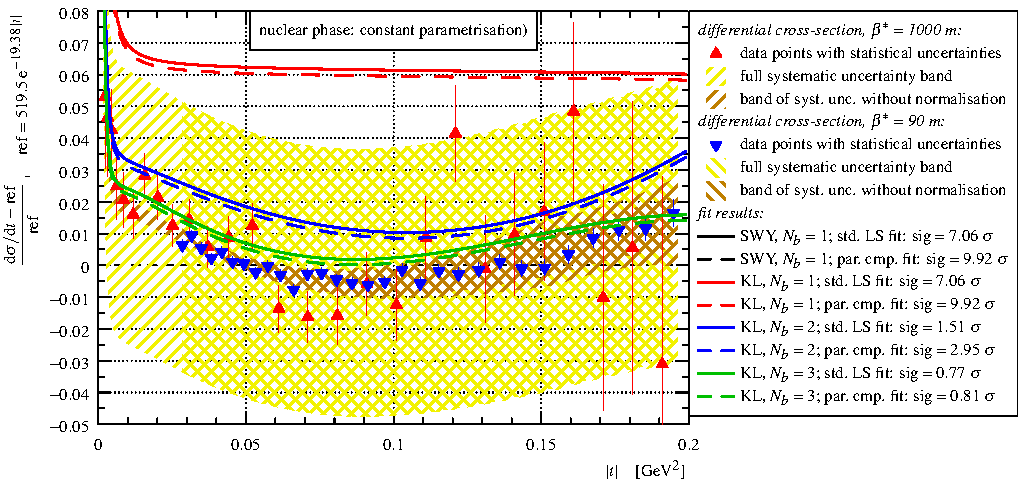
\includegraphics{fig/fits_common_con.pdf}
\caption{\TODO{caption}, only $p_0$ variable in phase}
\label{fig:fits common con}
\end{center}
\end{figure*}

\> Figure \ref{fig:fits common per}
\>> again, std LS and par cmp fits very similar (up to small difference in normalisation for $N_b = 1$)
\>> all fits reasonable

\begin{figure*}
\begin{center}
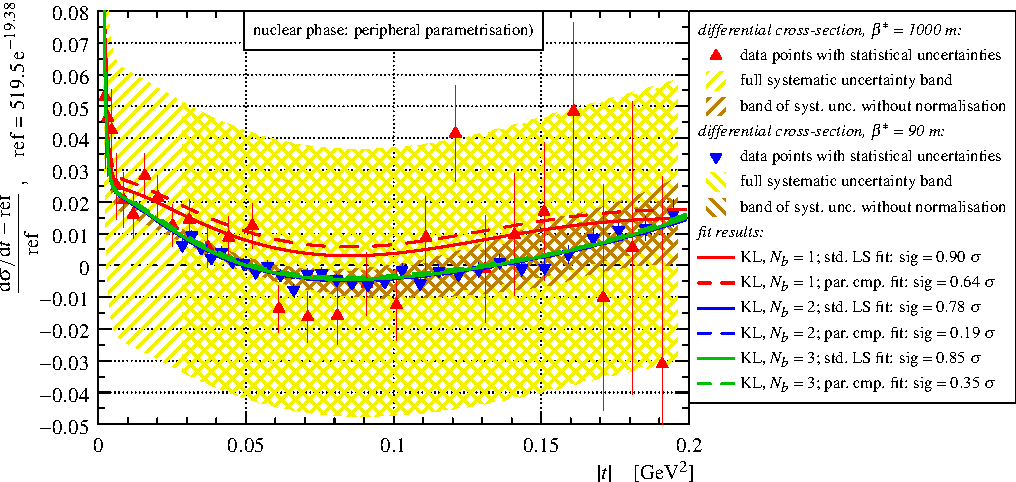
\includegraphics{fig/fits_common_per.pdf}
\caption{\TODO{caption}, all phase parameters variable}
\label{fig:fits common per}
\end{center}
\end{figure*}

\> Table \ref{tab:fits common}: parameters derived from fits shown in Figures~\ref{fig:fits common con} and \ref{fig:fits common per}
\>> \TODO{trends in data? Explain!}
\>> \TODO{illustrative decomposition of uncertainties from MC}
\>> visualised in Figure~\ref{fig:fits reciprocal der} (black points)


\begin{table*}
\caption{%
\TODO{caption}, parcmp fits as in Figures~\ref{fig:fits common con} and \ref{fig:fits common per}
}%
\label{tab:fits common}
\begin{center}
\small
\setlength{\tabcolsep}{5pt}
%\def\arraystretch{0.8}
\begin{tabular}{c@{\hskip20pt}cc@{\hskip20pt}cc}
\hline
\hline
% header
	& \multispan2\hfil constant \hfil & \multispan2\hfil peripheral \hfil  \cr
\hline
 			& $\rho = -0.027 \pm 0.021$ & $\sqrt{\langle b^2\rangle_{\rm el}} = 0.87\un{fm}$					& $\rho = 0.083 \pm 0.023$ & $\sqrt{\langle b^2\rangle_{\rm el}} = 1.68\un{fm}$					\cr
$N_b = 1$	& $B = (19.39 \pm 0.05)\un{GeV^{-2}}$ & $\sqrt{\langle b^2\rangle_{\rm inel}} = 1.34\un{fm}$		& $B = (19.68 \pm 0.07)\un{GeV^{-2}}$ & $\sqrt{\langle b^2\rangle_{\rm inel}} = 1.03\un{fm}$		\cr
			& $\sigma_{\rm tot} = (103.8 \pm 2.1)\un{mb}$ & $\sqrt{\langle b^2\rangle_{\rm tot}} = 1.23\un{fm}$	& $\sigma_{\rm tot} = (102.8 \pm 2.1)\un{mb}$ & $\sqrt{\langle b^2\rangle_{\rm tot}} = 1.24\un{fm}$	\cr\hline
%                                                                                                                                                                                                                   
 			& $\rho = 0.059 \pm 0.021$ & $\sqrt{\langle b^2\rangle_{\rm el}} = 0.87\un{fm}$						& $\rho = 0.120 \pm 0.026$ & $\sqrt{\langle b^2\rangle_{\rm el}} = 1.90\un{fm}$						\cr
$N_b = 2$	& $B = (19.97 \pm 0.07)\un{GeV^{-2}}$ & $\sqrt{\langle b^2\rangle_{\rm inel}} = 1.36\un{fm}$		& $B = (20.46 \pm 0.44)\un{GeV^{-2}}$ & $\sqrt{\langle b^2\rangle_{\rm inel}} = 0.96\un{fm}$		\cr
			& $\sigma_{\rm tot} = (102.8 \pm 2.1)\un{mb}$ & $\sqrt{\langle b^2\rangle_{\rm tot}} = 1.25\un{fm}$	& $\sigma_{\rm tot} = (104.13 \pm 2.3)\un{mb}$ & $\sqrt{\langle b^2\rangle_{\rm tot}} = 1.28\un{fm}$	\cr\hline
%                                                                                                                                                                                                                   
 			& $\rho = 0.090 \pm 0.024$ & $\sqrt{\langle b^2\rangle_{\rm el}} = 0.87\un{fm}$						& $\rho = 0.115 \pm 0.026$ & $\sqrt{\langle b^2\rangle_{\rm el}} = 2.01\un{fm}$						\cr
$N_b = 3$	& $B = (20.39 \pm 0.14)\un{GeV^{-2}}$ & $\sqrt{\langle b^2\rangle_{\rm inel}} = 1.37\un{fm}$		& $B = (20.04 \pm 0.36)\un{GeV^{-2}}$ & $\sqrt{\langle b^2\rangle_{\rm inel}} = 0.82\un{fm}$		\cr
			& $\sigma_{\rm tot} = (102.5 \pm 2.1)\un{mb}$ & $\sqrt{\langle b^2\rangle_{\rm tot}} = 1.26\un{fm}$	& $\sigma_{\rm tot} = (103.5 \pm 2.2)\un{mb}$ & $\sqrt{\langle b^2\rangle_{\rm tot}} = 1.25\un{fm}$	\cr\hline
\hline
\hline
\end{tabular}
\end{center}
%\vskip-10mm
\end{table*}



%----------------------------------------------------------------------------------------------------
\subsection{Reciprocally constrained 1000 and 90m fits}


\begin{figure*}
\begin{center}
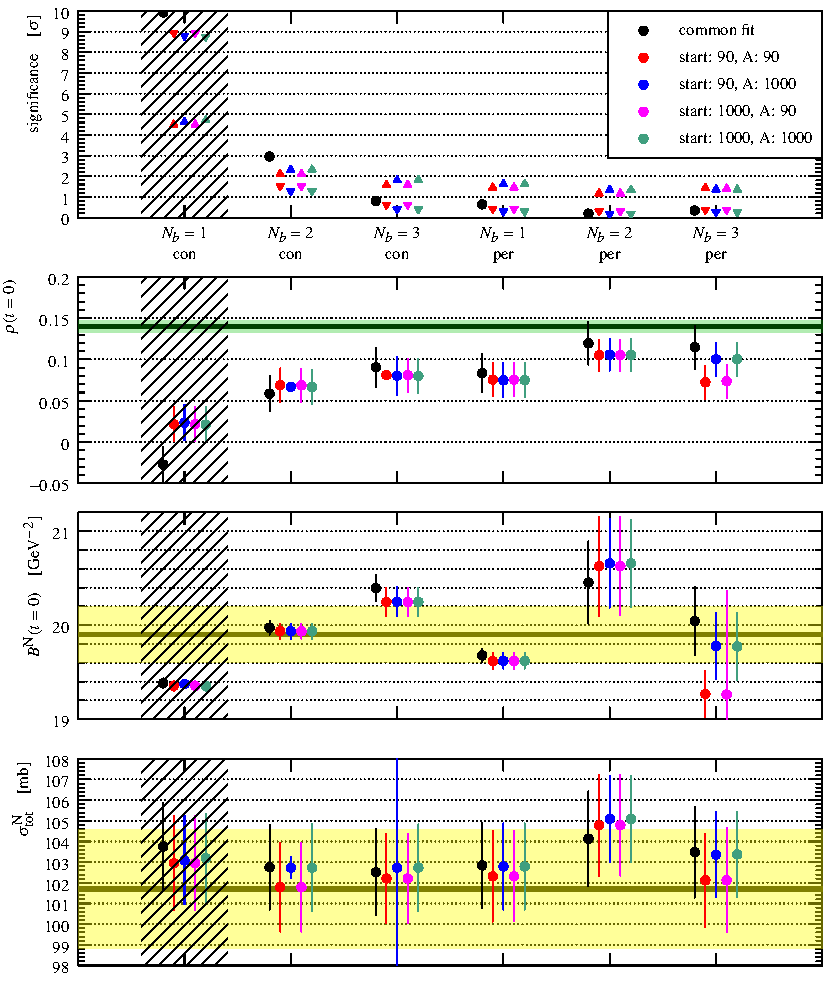
\includegraphics{fig/fits_reciprocal_derived.pdf}
\caption{\TODO{caption}
Points as in legend, black ones correspond to the results of Table~\ref{tab:fits common}. Significance: triangles up (down) from 1000m (90m) fit. Describe columns -- combinations of $N_b$ and phase parametrisation. The column $N_b=1$ and constant phase is hatched since this combination is excluded by the data. Yellow horizontal bands: results from PRL, reference to the delicate B comparison above? Green horizontal band: extrapolation by COMPETE - which one? Peripheral fits -- shape variable or fixed?
}
\label{fig:fits reciprocal der}
\end{center}
\end{figure*}
